%<dscrpt>Introduction aux fonctions d'une variable complexe. Théorème de Rouché</dscrpt>
Ce texte introduit\footnote{d'après W. Rudin \emph{Analyse réelle et complexe} Masson} aux fonctions d'une variable complexe à valeurs complexes mais les seules fonctions de ce type intervenant dans ce problème sont la fonction exponentielle complexe et des fonctions polynomiales ou rationnelles. On conviendra d'identifier un polynôme ou une fraction rationelle avec la fonction qui lui est associée. 

Ce texte fait aussi intervenir des fonctions $\mathcal{C}^{\infty}(\R)$, périodiques de période $2\pi$ et à valeurs dans $\C$. De telles fonctions sont appelées des \emph{lacets}. Une lacet $\gamma$ peut être vu comme un mouvement. Pour $t\in \R$, le complexe $\gamma(t)$ représente la position dans le plan d'un point mobile. La trajectoire (notée $\Gamma$) est l'ensemble des points par où est passé le mobile. \`A cause de la périodicité,
\[
 \Gamma = \left\lbrace \gamma(t), \; t\in \R \right\rbrace = \left\lbrace \gamma(t), \; t\in [0, 2\pi] \right\rbrace .
\]
Les figures \ref{fig: Erouche_1} et \ref{fig: Erouche_2} présentent les trajectoires $\Gamma$ pour deux lacets.
\begin{figure}[h]
  \centering
  \subfloat[$\gamma(t) = e^{it}$.\label{fig: Erouche_1}]{
    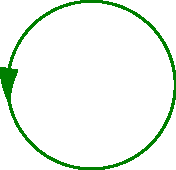
\includegraphics{./Erouche_1.pdf}
  }
  \hspace{3cm}
  \subfloat[$\gamma(t)=P(e^{it})$ avec $P=X^2 - X - 1$.\label{fig: Erouche_2}]{
    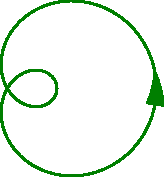
\includegraphics{./Erouche_2.pdf}
  }
  \caption{Exemples de trajectoires.}
\end{figure}

Pour une fonction $\gamma$ et $z\in \C \setminus \Gamma$, \emph{l'indice} de $z$ par rapport à $\Gamma$ est 
\[
 I_\gamma (z) = \frac{1}{2 i \pi}\int_{0}^{2\pi}\frac{\gamma'(t)}{\gamma(t) - z} \, dt.
\]
Il s'agit de l'intégrale d'une fonction d'une variable réelle $\mathcal{C}^{\infty}$ à valeurs complexes où $\gamma'(t)$ est la notation habituelle pour la dérivée de $\gamma$. Pour un nombre complexe $z$ tel que $|z|\neq 1$, on note $I_0(z)$ son indice par rapport au mouvement circulaire.
\[
 I_0(z) = \frac{1}{2  \pi}\int_{0}^{2\pi}\frac{ e^{it}}{e^{it} - z} \, dt\hspace{0.5cm} \text{avec } \gamma(t) = e^{it}.
\]
On rappelle que si $f$ est une fonction continue dans $[a,b]$ (avec $a < b$) à valeurs complexes,
\[
 \left| \int_a^b f(t)\, dt \right| \leq \int_a^b |f(t)|\, dt.
\]

\textbf{Remarques}. La partie V est totalement indépendante des autres parties. Les parties I et II ne dépendent pas l'une de l'autre mais prouvent la même proposition de deux manières différentes. La partie III n'utilise pas la proposition prouvée en I ou II. La partie IV utilise cette proposition ainsi que d'autres démontrées en III.

\subsection*{Partie préliminaire.}
\begin{enumerate}
 \item Soit $f$ continue dans $\R$, périodique de période $T>0$ et à valeurs complexes.\newline
Montrer que la fonction de $\R$ dans $\C$, $ x \mapsto \int_x^{x+T}f(t)\, dt$ est constante.

 \item Montrer que:
\[
 \forall x \in \R^*, \; \arctan x + \arctan \frac{1}{x} =
 \left\lbrace 
 \begin{aligned}
  \frac{\pi}{2} &\text{ si } x > 0 \\
  -\frac{\pi}{2} &\text{ si } x < 0
 \end{aligned}
 \right. .
\]

 \item Soit $z=|z|e^{i\varphi} \in \C$ avec $|z|\neq 1$ et $\varphi \in \R$. Pour tout $t\in \R$, exprimer 
\[
 (|z|-1)^2 - \left|e^{it} - z\right|^2
\]
en fonction de $t-\varphi$. En déduire
\[
\forall t \in \R, \; \left|e^{it} - z\right| \geq
\left\lbrace 
\begin{aligned}
 1 - |z| &\text{ si } |z| < 1 \\
 |z| - 1 &\text{ si } |z| > 1
\end{aligned}
\right. .
\]

\end{enumerate}

\subsection*{Partie I. Calcul direct de $I_0(z)$.}
Dans cette partie, $z \in \C$, $|z|\neq 1$ et $\varphi\in \R$ est un argument de $z$. On note
\[
 A(z) = \Re(I_0(z)), \hspace{1cm} B(z) = \Im(I_0(z)).
\]
\begin{enumerate}
 \item Soit $r \in \R \setminus\left\lbrace -1, +1 \right\rbrace$. Montrer que
\[
 \int_0^{\frac{\pi}{2}}\frac{d\theta}{1+r^2 - 2r\cos \theta}
 =
 \frac{2}{1-r^2}\arctan\left( \frac{1 + r}{1 - r}\right) .
\]

 \item 
 \begin{enumerate}
  \item  Montrer que
\[
 A(z) = \frac{1}{2\pi}\int_{0}^{2\pi}\frac{1 - |z| \cos(t-\varphi)}{1 + |z|^2 - 2|z|\cos(t-\varphi)}\, dt.
\]
  \item Montrer que 
\[
 I_0(z) = A(z) = \frac{1}{2} + 
 \frac{1-|z|^2}{4\pi}
 \int_0^{2\pi}\frac{dt}{1 + |z|^2 - 2|z|\cos(t-\varphi)}.
\]
 \end{enumerate}

  \item Montrer que
\begin{multline*}
 \int_0^{2\pi}\frac{dt}{1 + |z|^2 - 2|z|\cos(t-\varphi)} = \\
 2\left( 
 \int_0^{\frac{\pi}{2}}\frac{d\theta}{1 + |z|^2 - 2|z|\cos \theta}
 +
 \int_0^{\frac{\pi}{2}}\frac{d\theta}{1 + |z|^2 + 2|z|\cos \theta}
 \right) .
\end{multline*}
En déduire
$
I_0(z)=
\left\lbrace 
\begin{aligned}
 1 &\text{ si } |z| < 1\\
 0 &\text{ si } |z| > 1
\end{aligned}
\right. 
$.
\end{enumerate}

\subsection*{Partie II. Calcul de $I_0(z)$ avec une progression géométrique.}
\begin{enumerate}
 \item Soit $k\in \Z^*$, calculer $\int_{0}^{2\pi}e^{ikt}\, dt$.
 \item Dans cette question $|z| < 1$.
 \begin{enumerate}
  \item Montrer que:
\[
 \forall n \in \N, \; I_0(z) = 1 + \frac{z^{n+1}}{2\pi} \int_{0}^{2\pi} \frac{e^{-i(n+1)t}}{1-e^{-it}z}\, dt.
\]
  \item En déduire $I_0(z) = 1$.
 \end{enumerate}

 \item Dans cette question $|z| > 1$.
 \begin{enumerate}
  \item Montrer que:
\[
 \forall n \in \N, \; I_0(z) =  \frac{z^{-(n+1)}}{2\pi}\int_0^{2\pi}\frac{e^{i(n+2)t}}{e^{it} - z}\, dt.
\]
  \item En déduire $I_0(z) = 0$.
 \end{enumerate}
\end{enumerate}

\subsection*{Partie III. Propriétés de l'indice.}
Dans cette partie, $\gamma$ est un lacet et $z$ est un nombre complexe qui n'est pas sur la trajectoire: $z\notin \Gamma$.
\begin{enumerate}
 \item Dans cette question seulement, on considère l'équation différentielle
\begin{equation*}
 (\gamma - z) y' - \gamma' y = 0
\end{equation*}
où la fonction inconnue $y$ est à valeurs complexes.
\begin{enumerate}
 \item Déterminer la solution évidente qui prend en $t=0$ la valeur $\gamma(0) - z$.
 \item En utilisant un résultat de cours cité précisément, exprimer cette solution avec la fonction exponentielle complexe et une intégrale.
 \item Montrer que $I_\gamma(z) \in \Z$.
\end{enumerate}

 \item Dans cette question, pour $z$ et $z'$ en dehors de $\Gamma$, on cherche à majorer $\left| I_\gamma(z) - I_\gamma(z')\right|$.
 \begin{enumerate}
  \item Justifier l'existence d'un réel strictement positif noté $d(z,\Gamma)$ et défini par:
\[
 d(z,\Gamma) = \min \left\lbrace \left| z - \gamma(t) \right|, t\in [0, 2\pi ] \right\rbrace .
\]
  \item Montrer que $\left| I_\gamma(z) - I_\gamma(z')\right| \leq K \left| z - z' \right|$ avec 
\[
 K = \frac{\overline{\gamma}}{d(z,\Gamma)\,d(z',\Gamma)} \hspace{0.5cm} \text{ et } \hspace{0.5cm} \overline{\gamma} = \frac{1}{2\pi} \int_{0}^{2\pi}\left|\gamma'(t)\right|\, dt.
\] 

 \end{enumerate}
\begin{figure}[h]
 \centering
 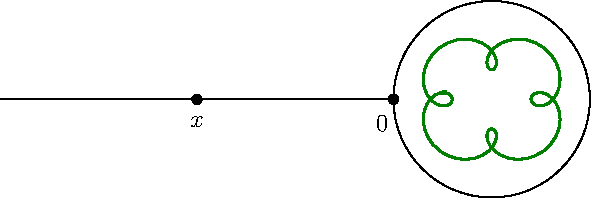
\includegraphics{./Erouche_3.pdf}
 % Erouche_3.asy: 0x0 pixel, 478dpi, 0.00x0.00 cm, bb=
 \caption{Configuration de la trajectoire pour la question \ref{trajdisq}.}
 \label{fig:rouche_3}
\end{figure}

\item \label{trajdisq}
 Dans cette question, on suppose que $\Gamma$ est dans le disque ouvert de rayon $
 1$ et de centre $1$ c'est à dire que 
\[
 \forall t \in \R, \; \left| \gamma(t) - 1 \right| < 1.
\]
\begin{enumerate}
 \item Montrer que $]-\infty , 0 ] \cap \Gamma = \emptyset$. Montrer que, pour tout $x \leq 0$,
\[
 d(x,\Gamma) > |x| \; \text{ et } \; d(x,\Gamma) \geq d(0,\Gamma).
\]

 \item Montrer que la restriction de $I_\gamma$ à $]-\infty, 0]$ est lipschitzienne de rapport $\frac{4 \, \overline{\gamma}}{d(0,\Gamma)^2}$.
 \item Montrer que $\left|I_\gamma(x)\right| \leq \frac{\overline{\gamma}}{|x|}$ pour $x<0$.
 \item Montrer que $I_\gamma(0) = 0$.
\end{enumerate}

\end{enumerate}

\subsection*{Partie IV. Nombre de racines.}
\begin{enumerate}
 \item Dans cette question, $P\in \C[X]$ est un polynôme de degré au moins $1$ sans racine de module 1 et on considère un lacet $\gamma_P$ définit par 
\[
 \forall t \in \R, \; \gamma_P(t) = P(e^{it}).
\]
On note $z_1, \cdots, z_s$ les racines de $P$ et $m_1, \cdots, m_s$ leurs multiplicités.\newline
Montrer que
\[
 I_{{\gamma}_P}(0) = \sum_{k=1}^{s}m_kI_0(z_k).
\]
En déduire que $I_{\gamma_P}(0)$ est la somme des multiplicités de racines de $P$ dans le disque unité ouvert.

 \item Théorème de Rouché\footnote{d'après une idée de mon ami Saman K.}.\newline
 Soit $P$ et $Q$ dans $\C[X]$ non constants et n'admettant aucune racine de module $1$. On définit un lacet $\gamma$ par :
\[
 \forall t \in \R, \; \gamma(t) = \frac{P(e^{it})}{Q(e^{it})}.
\]

\begin{enumerate}
  \item Montrer que $I_\gamma(0) = I_{\gamma_P}(0) - I_{\gamma_Q}(0)$.
  \item On suppose de plus que $\left|P(e^{it}) - Q(e^{it})\right| < \left| Q(e^{it}) \right|$ pour tout $t$ réel.\newline
 Montrer que $I_{\gamma_P}(0) = I_{\gamma_Q}(0)$.
\end{enumerate}

 \item Pour tout $n\in \N^*$, on définit
\[
 P = X^n(X^2 - X - 1) + X^2 -1 \; \text{ et } \; Q = X^n(X^2 - X - 1).
\]
\begin{enumerate}
 \item En utilisant $e^{it} - e^{-it} = 2i \sin t$, montrer que 
\[
 \forall t \in \R, \; \left| \frac{(e^{it})^2 - 1}{(e^{it})^n\left( (e^{it})^2 - e^{it} - 1\right) }\right| < 1.
\]
  \item Montrer que $I_{\gamma_P}(0) = I_{\gamma_Q}(0)$.
  \item Montrer que $P$ admet une racine réelle strictement plus grande que $1$ et que la somme des multiplicités de ses racines dans le disque unité ouvert est $n+1$.
\end{enumerate}
\end{enumerate}

\subsection*{Partie V. Harmonicité. Formule de Cauchy.}
\begin{enumerate}
 \item Montrer que, pour tout lacet $\gamma$ et tout polynôme $Q\in \C[X]$, 
\[
 \int_{0}^{2\pi}Q(\gamma(t))\gamma'(t)\,dt = 0.
\]
 \item Soit $z\in \C$ et $\gamma$ le lacet défini par $\gamma(t) = z + e^{it}$.\newline Quelle est la trajectoire de $\gamma$? Montrer que
\[
 \frac{1}{2\pi}\int_0^{2\pi}P(\gamma(t))\,dt = \frac{1}{2i\pi}\int_0^{2\pi}\frac{P(\gamma(t))}{\gamma(t) - z}\,\gamma'(t)\,dt = P(z).
\]

\end{enumerate}



